\documentclass[12pt]{article}
% set tiems new roman in latex
\usepackage{newtxtext}
\usepackage[paper=letterpaper,margin=2.54cm]{geometry}
\usepackage{amsmath}
\usepackage{amssymb}
\usepackage{amsfonts}
\usepackage{newtxtext, newtxmath}
% \usepackage{enumitem}
\usepackage{enumerate}
\usepackage{titling}
\usepackage[colorlinks=true]{hyperref}
\usepackage{graphicx}
\usepackage{float}
\usepackage{listings}
\usepackage{xcolor}
\usepackage{color}
\usepackage{caption}
\usepackage{subfigure}
\usepackage{float}
\usepackage{booktabs}
\usepackage{multirow}

% citation
\usepackage[numbers]{natbib}

\setlength{\droptitle}{-6em}
% Enter the specific assignment number and topic of that assignment below, and replace "Your Name" with your actual name.
\title{Project: Comp 6771 Image Processing}
\author{Yunqi Xu 40130514}
\date{\today}


\begin{document}
% \maketitle
\begin{titlepage}
  \rule{\textwidth}{1pt}   % The top horizontal rule
    \vspace{0.2\textheight}  % Whitespace between top horizontal rule and title

    %------------------------------------------------------------
    %    Title
    %------------------------------------------------------------

    {\Huge COMP 6771 Image Processing: Project}

    \vspace{0.025\textheight}   % Whitespace between the title and short horizontal rule

    \rule{0.83\textwidth}{0.4pt}  % The short horizontal rule under title

    \vspace{0.1\textheight}  % Whitespace between the short horizontal rule and author

    %------------------------------------------------------------
    %    Author
    %------------------------------------------------------------

    {\Large Student name: \textsc{Yunqi Xu}}
    \vfill
    {\Large Student id: 40130514}
    \vfill  % Whitespace between author and date

    {\large \today}
    \vspace{0.1\textheight}  % Whitespace between date and bottom horizontal rule

    %------------------------------------------------------------
    %    Bottom rules
    %------------------------------------------------------------

    \rule{\textwidth}{1pt}  % The bottom horizontal rule
\end{titlepage}

\section{Introduction}
\subsection{Bilateral filter and Gaussian adaptive bilateral filter}
\label{subsection review bilateral}
% overall summary of bilateral filter
Bilateral filter was proposed by Tomasi in 1998~\cite{paper_bf}, Which is edges keeping, noises removing, simple and non-iterative,multi-channels suitable method, consisted by two filters, Geometric closeness(domain filter $c(\xi, x)$ and photometric similarity(range filter $s(\xi, x)$).  
% Bilateral filter is an angorithm which is nonlinear, edges perserving and Gaussian denoising method proposed by Tomasi in 1998[cite]. 

% Bilateral filter utilizes two gaussian like filter, geometric closeness and pholometric similarity, to solve the problem 

% review of the bilateral filter method
% The main method that the bilateral filter utilized are two Gaussian filters. 
% One is calcualted based on the Geometric closeness. 
% Another is calculated based on their photometric similarity
% Below is the process of Bilateral Filtering an image:
% add the processing step

% achievement
% The process of Bilateral filter is shown blow:





% \subsection{Review of another paper}
% In this section, first introduce another method that provided by other paper, and then compared with the Bilateral filter

\begin{figure}[H]
  \centering
  \subfigure[Processing of Bilateral filter]{
  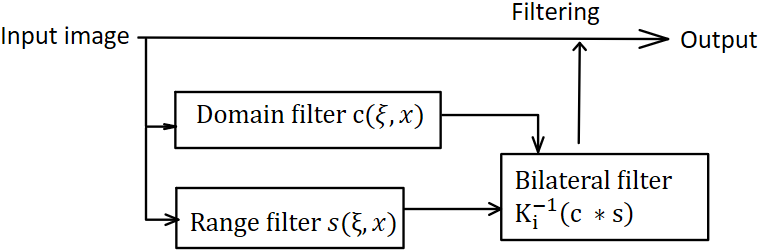
\includegraphics[width=7cm]{cite images/1.png}
  % \caption{fig1}
  \label{processing_bf}
  }
  \quad
  \subfigure[Processing Gaussian adaptive bilaterl filter]{
  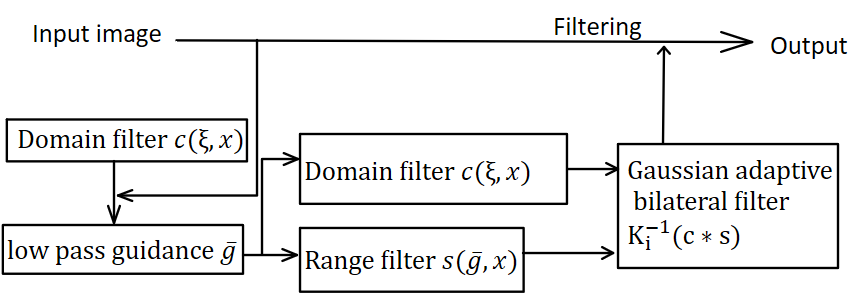
\includegraphics[width=7cm]{cite images/2.png}
  \label{processing_gabf}
  }
\caption{Comparison between Bilateral filter and Gaussian adaptive Bilater filter}
\label{processing}
\end{figure}

The process of utilizing Bilater filter denoising an image is presented in Fig.~\ref{processing_bf}, where the Domain filter $c(\xi, x) = e^{-\frac{1}{2}(\frac{d(\xi, x)}{\sigma_{d}})^2}$,  where, $d(\xi, x)$ is the Euclidean distance between $\xi$ and $x$. The Range filter $s(\xi, x) = e^{-\frac{1}{2}(\frac{\delta(f(\xi), f(x))}{\sigma_{r}})^{2}}$, where, $\delta(\phi, f)$ is a suitable measure of distance between the two intensity value $\phi$ and f. Also the $K_i^{-1}$ denotes a normalizing factor.
The overall processing could be descrbed as using the weighted sum of multiple of two generated gaussian-like kernel filtering an input image.



% \begin{enumerate}[Step1:]
% \item Calculate Domain filter based on the $\sigma_d$ and $k\_size$, 
% \item for a certain position $(x, y)$ in an input image, calculate Range filter based on the $\sigma_r$, $k\_size$ and input image, 
% \item Calculate the sum of mutiple between domain filter * range filter with a pitch($size = k\_size * k\_size)$ of input image which the center is $(x, y)$ to fet a new value of (x, y).
% \item Repeat Step 2 and Step 3 until all pixel are visited. 
% \end{enumerate}

The Bilateral filter can significantly solve the slow spatial variantion fails at edges, which usually occurs with tranditional Gaussian filters, and the complexity of many iteration that brought by Diffusion method. 
The result in the Bilateral filter~\cite{paper_bf} indicates that it is suitable from both gray and color images. 
However, in the evluation of the paper, the lack of quantitive comparison between bilateral filter and other baseline method make it difficult to generate though with readers.

On the other hand, another improvement version of Bilateral filter, Gaussian adaptive bilaterl filter, purposed by Chen~\cite{9200678} in 2020, which using two nonindentical filters solving the inherent problem occured in Gaussian range filter when facing a noise filtering input and its effect on edge-preserving image smoothing operation. 

The process of Gaussian adaptive bilateral filter is in Fig.~\ref{processing_gabf}
The same as the processof Bilateral filter, the GABF use two filters, domain filter and range filter, however, the compared with BF in Fig.~\ref{processing_bf}, the range filter is generated with a pre-calculation low pass guidence $\bar{g}$ with Gaussian domain filter. 
So the Range filter will calculate the intensity difference between input image and $\bar{g}$.

The result in~\cite{9200678}, indicates the succseeful of the GABF, and also the auther use quantivative analysis such as the SSIM, PSNR and GMSD to evaluate its output, all of the output is achieve advantages compared with BF.

\bibliographystyle{IEEEtranN}
\bibliography{reference}


\clearpage
\section{Details of Bilateral Filter}
\label{section Bilateral_filter}
% modify with citation of sections
This section contains three main parts. we will firstly present the result of our re-implement method, and then compared the bilater filter with other baseline algorithm in terms of other low pass filters that usually blur the image but also blur edges. 
Finally, we will discuss about the Bilateral filter from both advantages and disadvantages and the difficulties during the implement process.


\subsection{Result of the Re-implement algorithm}
\label{section reimplement}
The main purpose for this section is providing an provement of the successful re-implement of the Bilateral filter.
During our experiment, we use the images from the Bilateral filter paper~\cite{paper_bf}, inputted the same parameters that the paper utilized, and compared our result with the oroginal paper and also the build-in function with Opencv-python offcial to prove the successfully re-implement of our code.

\subsubsection{Test result on gray images}
\label{subsection test gray}
Firstly, we present our result compared with the result indicated in the paper, with the same inputted parameters and the same pattern.
In the papre, the author use the parameters $\sigma_d = (1, 3, 10)$ and $\sigma_r = (10, 30, 100, 300)$ correspond to each consisting the parameter set.  
We also use the $kernel\_size = 25$.
The Fig.~\ref{im_cateye} presents the output of our re-implement Bilateral filter.
In this Figure, we can find the blur trend are similar with Figure 3. from the Bilteral filter paper.
The Fig.~\ref{im_cateye_1_10} has the most clean result, but part of small noises still could be find in it. 
On the other hand, the Fig.~\ref{im_cateye_10_300} is the most blur one in these outputs, it only remain a blurry profile of the cat. 

\begin{figure}[H]
  \centering
  \subfigure[$\sigma_d=1, \sigma_r=10$]{
  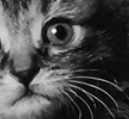
\includegraphics[width=3cm]{output_image/cat_part_ds1_rs10.png}
  % \caption{fig1}
  \label{im_cateye_1_10}
  }
  \quad
  \subfigure[$\sigma_d=1, \sigma_r=30$]{
  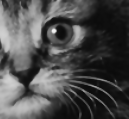
\includegraphics[width=3cm]{output_image/cat_part_ds1_rs30.png}
  }
  \quad
  \subfigure[$\sigma_d=1, \sigma_r=100$]{
  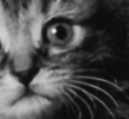
\includegraphics[width=3cm]{output_image/cat_part_ds1_rs100.png}
  }
  \quad
  \subfigure[$\sigma_d=1, \sigma_r=300$]{
  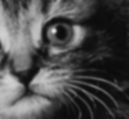
\includegraphics[width=3cm]{output_image/cat_part_ds1_rs300.png}
  }

  \subfigure[$\sigma_d=3, \sigma_r=10$]{
  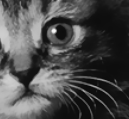
\includegraphics[width=3cm]{output_image/cat_part_ds3_rs10.png}
  % \caption{fig1}
  }
  \quad
  \subfigure[$\sigma_d=3, \sigma_r=30$]{
  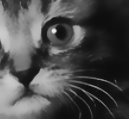
\includegraphics[width=3cm]{output_image/cat_part_ds3_rs30.png}
  }
  \quad
  \subfigure[$\sigma_d=3, \sigma_r=100$]{
  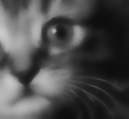
\includegraphics[width=3cm]{output_image/cat_part_ds3_rs100.png}
  }
  \quad
  \subfigure[$\sigma_d=3, \sigma_r=300$]{
  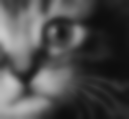
\includegraphics[width=3cm]{output_image/cat_part_ds3_rs300.png}
  }

  \subfigure[$\sigma_d=10, \sigma_r=10$]{
  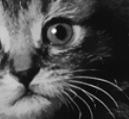
\includegraphics[width=3cm]{output_image/cat_part_ds10_rs10.png}
  % \caption{fig1}
  }
  \quad
  \subfigure[$\sigma_d=10, \sigma_r=30$]{
  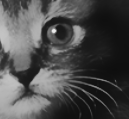
\includegraphics[width=3cm]{output_image/cat_part_ds10_rs30.png}
  }
  \quad
  \subfigure[$\sigma_d=10, \sigma_r=100$]{
  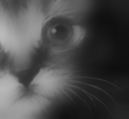
\includegraphics[width=3cm]{output_image/cat_part_ds10_rs100.png}
  }
  \quad
  \subfigure[$\sigma_d=10, \sigma_r=300$]{
  
\includegraphics[width=3cm]{output_image/cat_part_ds10_rs300.png}
  \label{im_cateye_10_300}
  }
\caption{A detail figure with bilateral filters with various range and domain parameter values by implement code}
\label{im_cateye}
\end{figure}

As the comparison, we also make an experiment of input the same parameter pairs in to the build-in opencv-python funtion to explore whether it will have the same output as our code. Fig.~\ref{py_cateye} prove the results are samilar. 

\begin{figure}[b]
  \centering
  \subfigure[$\sigma_d=1, \sigma_r=10$]{
  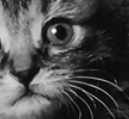
\includegraphics[width=3.5cm]{output_image_python/cat_part_ds1_rs10.png}
  % \caption{fig1}
  }
  \quad
  \subfigure[$\sigma_d=1, \sigma_r=30$]{
  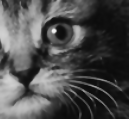
\includegraphics[width=3.5cm]{output_image_python/cat_part_ds1_rs30.png}
  }
  \quad
  \subfigure[$\sigma_d=1, \sigma_r=100$]{
  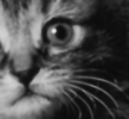
\includegraphics[width=3.5cm]{output_image_python/cat_part_ds1_rs100.png}
  }
  \quad
  \subfigure[$\sigma_d=1, \sigma_r=300$]{
  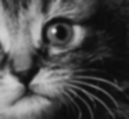
\includegraphics[width=3.5cm]{output_image_python/cat_part_ds1_rs300.png}
  }

  \subfigure[$\sigma_d=3, \sigma_r=10$]{
  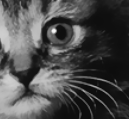
\includegraphics[width=3.5cm]{output_image_python/cat_part_ds3_rs10.png}
  % \caption{fig1}
  }
  \quad
  \subfigure[$\sigma_d=3, \sigma_r=30$]{
  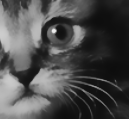
\includegraphics[width=3.5cm]{output_image_python/cat_part_ds3_rs30.png}
  }
  \quad
  \subfigure[$\sigma_d=3, \sigma_r=100$]{
  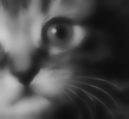
\includegraphics[width=3.5cm]{output_image_python/cat_part_ds3_rs100.png}
  }
  \quad
  \subfigure[$\sigma_d=3, \sigma_r=300$]{
  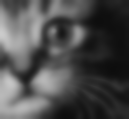
\includegraphics[width=3.5cm]{output_image_python/cat_part_ds3_rs300.png}
  }

  \subfigure[$\sigma_d=10, \sigma_r=10$]{
  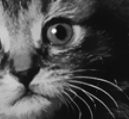
\includegraphics[width=3.5cm]{output_image_python/cat_part_ds10_rs10.png}
  % \caption{fig1}
  }
  \quad
  \subfigure[$\sigma_d=10, \sigma_r=30$]{
  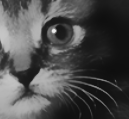
\includegraphics[width=3.5cm]{output_image_python/cat_part_ds10_rs30.png}
  }
  \quad
  \subfigure[$\sigma_d=10, \sigma_r=100$]{
  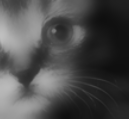
\includegraphics[width=3.5cm]{output_image_python/cat_part_ds10_rs100.png}
  }
  \quad
  \subfigure[$\sigma_d=10, \sigma_r=300$]{
  
\includegraphics[width=3.5cm]{output_image_python/cat_part_ds10_rs300.png}
  }
  \caption{A detail figure with bilateral filters with various range and domain parameter values by Opencv python}
  \label{py_cateye}
  \end{figure}
% Fig.~\ref{py_cateye} indicates that the similarity of output between our re-implement code and the build-in algorithm in python, in other ways prove the successful implement of our code. the output looks very similar.

\begin{figure}[H]
  \centering
  \subfigure[$\sigma_d=1, \sigma_r=10$]{
  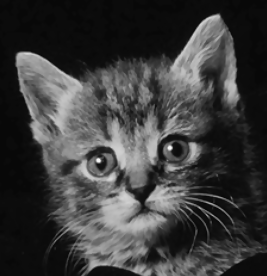
\includegraphics[width=3.5cm]{output_image/cat_ds1_rs10.png}
  % \caption{fig1}
  }
  \quad
  \subfigure[$\sigma_d=1, \sigma_r=30$]{
  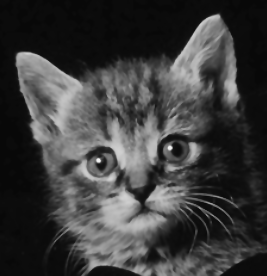
\includegraphics[width=3.5cm]{output_image/cat_ds1_rs30.png}
  }
  \quad
  \subfigure[$\sigma_d=1, \sigma_r=100$]{
  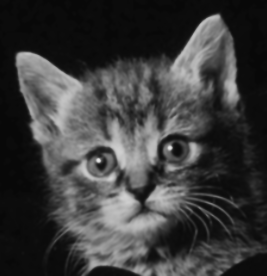
\includegraphics[width=3.5cm]{output_image/cat_ds1_rs100.png}
  }
  \quad
  \subfigure[$\sigma_d=1, \sigma_r=300$]{
  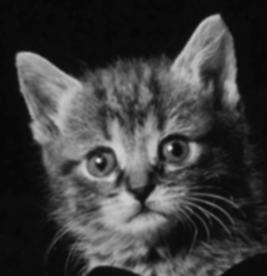
\includegraphics[width=3.5cm]{output_image/cat_ds1_rs300.png}
  }

  \subfigure[$\sigma_d=3, \sigma_r=10$]{
  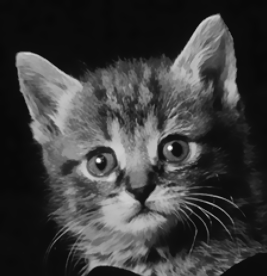
\includegraphics[width=3.5cm]{output_image/cat_ds3_rs10.png}
  % \caption{fig1}
  }
  \quad
  \subfigure[$\sigma_d=3, \sigma_r=30$]{
  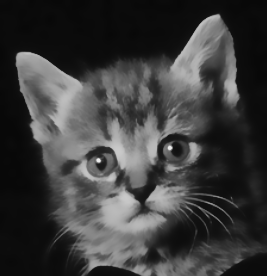
\includegraphics[width=3.5cm]{output_image/cat_ds3_rs30.png}
  }
  \quad
  \subfigure[$\sigma_d=3, \sigma_r=100$]{
  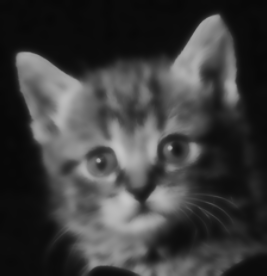
\includegraphics[width=3.5cm]{output_image/cat_ds3_rs100.png}
  }
  \quad
  \subfigure[$\sigma_d=3, \sigma_r=300$]{
  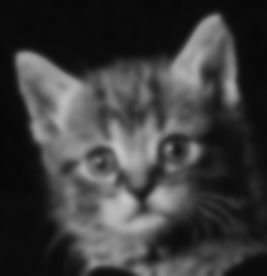
\includegraphics[width=3.5cm]{output_image/cat_ds3_rs300.png}
  }

  \subfigure[$\sigma_d=10, \sigma_r=10$]{
  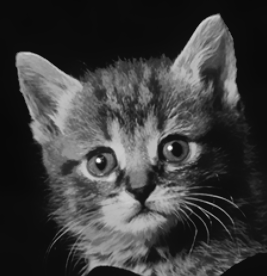
\includegraphics[width=3.5cm]{output_image/cat_ds10_rs10.png}
  % \caption{fig1}
  }
  \quad
  \subfigure[$\sigma_d=10, \sigma_r=30$]{
  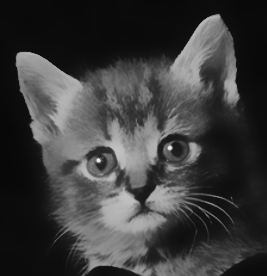
\includegraphics[width=3.5cm]{output_image/cat_ds10_rs30.png}
  }
  \quad
  \subfigure[$\sigma_d=10, \sigma_r=100$]{
  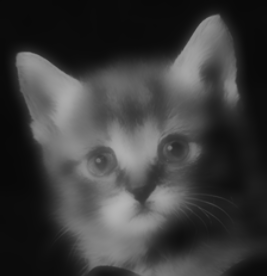
\includegraphics[width=3.5cm]{output_image/cat_ds10_rs100.png}
  }
  \quad
  \subfigure[$\sigma_d=10, \sigma_r=300$]{
  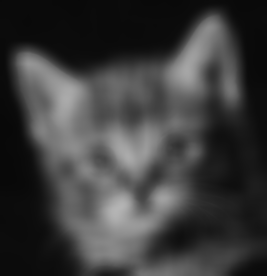
\includegraphics[width=3.5cm]{output_image/cat_ds10_rs300.png}
  }
  \caption{A detail figure with bilateral filters with various range and domain parameter values by re-implement code of cat}
  \label{im_cat}
  \end{figure}

Fig.~\ref{im_cat} are some other outputs use the cat image from paper and the same parameter sets. 
The same as the figures from the paper, some detils, such as the Kitten's whiskers, also can be remained after filtering.

% Fig.~\ref{im_cat} are also two image which prove the success of our re-implement code. 
The Fig.~\ref{snack} are some other outputs use the figures from Bilateral filter paper.  
The Fig.~\ref{snack_original}, ~\ref{snack_onion} are the oroginal images.
As present in Fig.~\ref{snack_original_smooth}, the salt and pepper noise can be removed, at the mean time, the edge information can be keeped as shown in Fig.~\ref{snack_onion_smooth}.
In this experiment, we use same parameters which the paper used. $\sigma_d = 3$ and $\sigma_r = 50$. 


\begin{figure}[H]
  \centering
  \subfigure[Original snack]{
  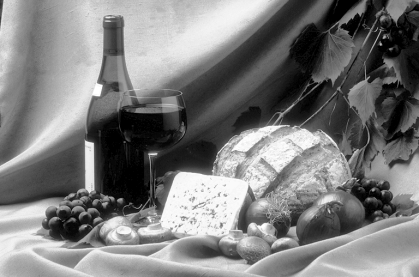
\includegraphics[width=6cm]{original_paper_images/gray/snack_a.png}
  \label{snack_original}
  }
  \quad
  \subfigure[Smoothed snack]{
  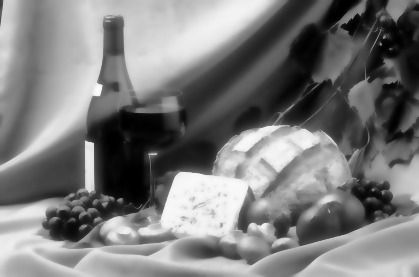
\includegraphics[width=6cm]{output_image/snack_a_ds2_rs50.png}
  \label{snack_original_smooth}
  }
  \quad
  \subfigure[Original Onion]{
  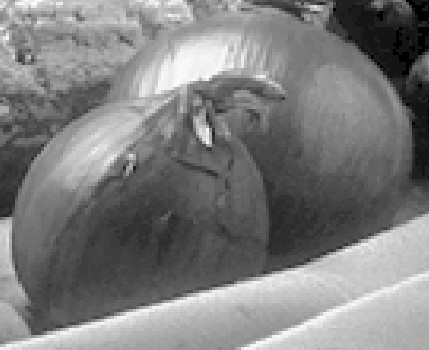
\includegraphics[width=4.5cm]{original_paper_images/gray/onion.png}
  \label{snack_onion}
  }
  \quad
  \subfigure[Smoothed Onion]{
  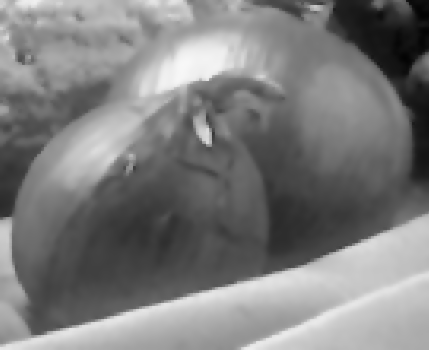
\includegraphics[width=4.5cm]{output_image/onion_ds3_rs50.png}
  \label{snack_onion_smooth}
  }
  \caption{The Bilater filtering result of snacks and the Onion detail}
  \label{snack}
\end{figure}

\subsubsection{Test result on color images}
The bilateral filter is not only suitable for filtering gray image, but also achieving successful at filtering color images.
Fig.~\ref{color} has presents the result of filtering on color images.
In these images, the left half (Fig.~\ref{color_children}, ~\ref{color_cube}, ~\ref{color_sky}, ~\ref{color_home})are original imput images.
The right half(Fig.~\ref{color_children_smooth}, ~\ref{color_cube_smooth}, ~\ref{color_sky_smooth} and~\ref{color_home_smooth}) are the result of those color images with Bilater filtering. 
Compared with filtering gray images, filtering color images need to convert 3-channels RGB images into the CIE-lab space, and then generate two filters based on geometric and photometric information that an image provided.
Noises on the original input images could be removed.

\begin{figure}[H]
  \centering
  \subfigure[Child]{
  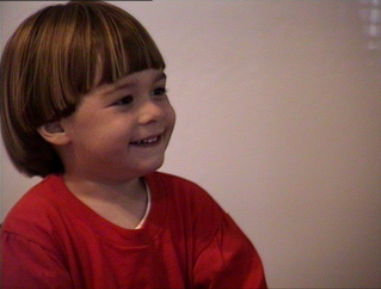
\includegraphics[width=6cm]{original_paper_images/color/child.png}
  \label{color_children}
  }
  \quad
  \subfigure[Smoothed Child]{
  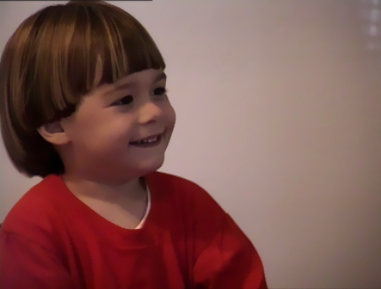
\includegraphics[width=6cm]{output_color_image/child_ds3_rs10.png}
  \label{color_children_smooth}
  }
  \caption{Output of child image}
  \label{color_child}
\end{figure}


\begin{figure}[H]
  \centering
  \subfigure[Rubik's cube]{
  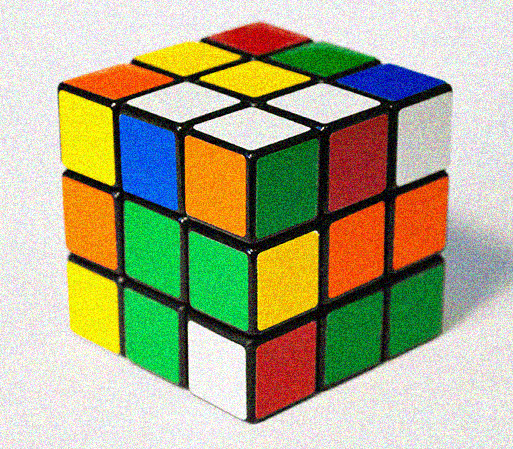
\includegraphics[width=4.5cm]{original_paper_images/color/rubiks_cube.png}
  \label{color_cube}
  }
  \quad
  \subfigure[Sky]{
  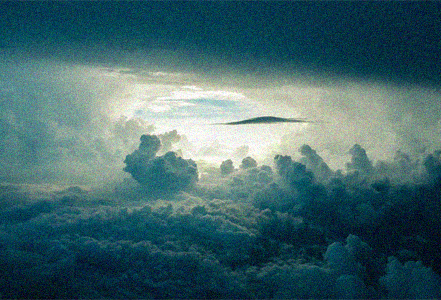
\includegraphics[width=4.5cm]{original_paper_images/color/sky.png}
  \label{color_sky}
  }
  \quad
    \subfigure[Home]{
    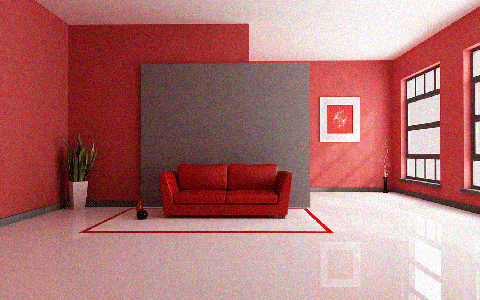
\includegraphics[width=4.5cm]{original_paper_images/color/home.png}
    \label{color_home}
    }
  \quad

  \subfigure[Smoothed Rubik's cube]{
  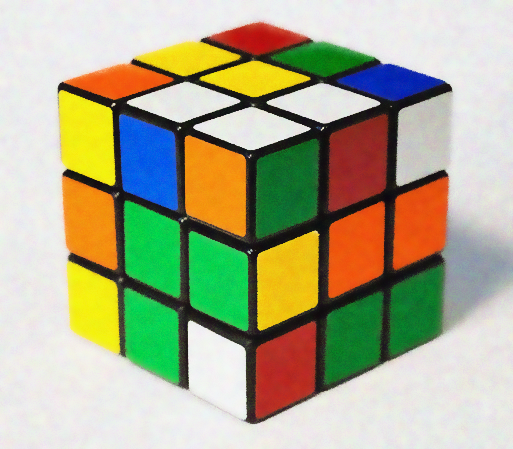
\includegraphics[width=4.5cm]{output_color_image/rubiks_cube_ds3_rs50.png}
  \label{color_cube_smooth}
  }
  \quad
  \subfigure[Smoothed sky]{
  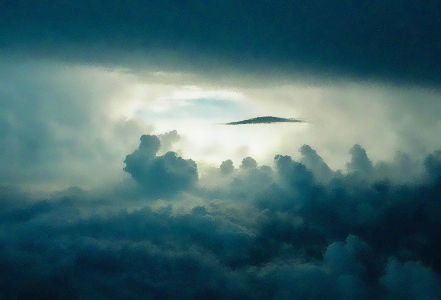
\includegraphics[width=4.5cm]{output_color_image/sky_ds3_rs30.png}
  \label{color_sky_smooth}
  }
  \quad
  \subfigure[Smoothed home]{
  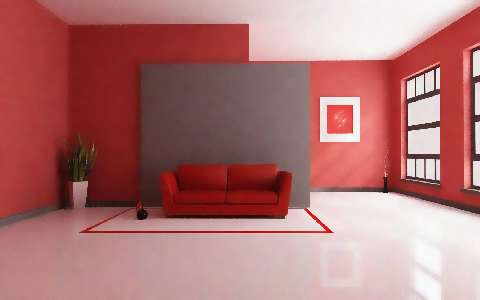
\includegraphics[width=4.5cm]{output_color_image/home_ds3_rs30.png}
  \label{color_home_smooth}
  }
  \caption{Outputs of other color images}
  \label{color}
\end{figure}

\subsection{Compare with other baseline algorithm}
\label{baseline comparison}
% in this section, compared with other blur algorithm
In this section, we compared the filter result of Bilateral filter with other baseline algorithm to present the advantages of our code.
The baseline low-pass filters we used are mean filtering, median filtering and gaussian filtering. 
All of this filters are classic filtering in terms of image processing.
The Section~\ref{section reimplement} not only prove the result of the re-implement code, but also indicate that the general applicability of Bilateral filter.
Our next experiment, we not only compared the output result passed by different filters from human version level, but also calculate the PNSR~\cite{paper_psnr} from mathmatical level. 
The equation of PNSR has been shwo in Eq.~\ref{PSNR equation}:
\begin{equation}
  PSNR = 10\log 10 (\frac{I_{Max}^{2}}{MSE})
  \label{PSNR equation}
\end{equation}

\begin{equation}
  MSE = \frac{\sum_{M, N}[I_1(m,n) - I_2(M, n)]^2}{M * N}
  \label{MSE}
\end{equation}

Where, the $I_{Max}$ is the maximum fluctuation in the input images. 
In our case, the 8-bit integer input image should have $R = 255$.
And the $I_1$ and $I_2$ are the two images between the noisey one and the filtered one.
  
\begin{figure}[H]
  \centering
  \subfigure[$Mean_{psnr}=19.89$]{
  \includegraphics[width=2.5cm]{output_baseline/cat_mean_23.png}
  \label{gray_baseline_mean}
  }
  \quad
  \subfigure[$Median_{psnr}=20.66$]{
  \includegraphics[width=2.5cm]{output_baseline/cat_median_23.png}
  \label{gray_baseline_median}
  }
  \quad
  \subfigure[Gaussian(1)]{
  \includegraphics[width=2.5cm]{output_baseline/cat_gaussian_23_ds_1.png}
  \label{gray_baseline_gaussian}
  }
  \quad
  \subfigure[Gaussian(3)]{
  \includegraphics[width=2.5cm]{output_baseline/cat_gaussian_23_ds_3.png}
  \label{gray_baseline_gaussian}
  }
  \quad
  \subfigure[Gaussian(10)]{
  \includegraphics[width=2.5cm]{output_baseline/cat_gaussian_23_ds_10.png}
  \label{gray_baseline_gaussian}
  }
  % \quad
  % \subfigure[Bilateral filter output]{
  % \includegraphics[width=3cm]{output_baseline/cat_ds3_rs30_ks_23.png}
  % \label{gray_baseline_bilateral}
  % }
  \caption{output compared with the baseline low pass filters}
  \label{gray_baseline}
\end{figure}

The Fig.~\ref{gray_baseline} has presented the result between three baseline filters and the Bilateral filter. 
Is is obvious that the the Fig.~\ref{gray_baseline_mean} and Fig.~\ref{gray_baseline_median} get a very bad result, since all the details and texture inforamtions are lose. 
The only remaining parts are the contour in each image.
The result of Gaussian filter, Fig.~\ref{gray_baseline_gaussian} can achieve a very closely result compared with Fig.~\ref{gray_baseline_bilateral}.
However, as we mentioned in Section.~\ref{subsection test gray}, the kitten's whiskers are clean in Fig.~\ref{gray_baseline_bilateral}, they are blured in Fig.~\ref{gray_baseline_gaussian}. 
For further prove our statement, we calculate the PSNR between each output image with filter and the original noisy image.
The Table.~\ref{table_PSNR} presents the PSNR result. 
As the result in the table, the PSNR scores of Median filter and Mean filter are too low to use, but the PSNR score of Gaussian filter can achieve a considerablely compititive result as 31.59, which is higher than using Bilateral filter with $\sigma_s = 3$ and $\sigma_d = 100$ or $\sigma_d = 300$ and $\sigma_s = 10$ and $\sigma_d = 30, 100, 300$. 

\begin{figure}[H]
  \centering
  \subfigure[$Mean_{psnr}=26.12$]{
  \includegraphics[width=2.5cm]{output_baseline/child_mean_23.png}
  \label{gray_baseline_mean}
  }
  \quad
  \subfigure[$Median_{psnr}=28.59$]{
  \includegraphics[width=2.5cm]{output_baseline/child_median_23.png}
  \label{gray_baseline_median}
  }
  \quad
  \subfigure[Gaussian(1)]{
  \includegraphics[width=2.5cm]{output_baseline/child_gaussian_23_ds_1.png}
  \label{gray_baseline_gaussian}
  }
  \quad
  \subfigure[Gaussian(3)]{
  \includegraphics[width=2.5cm]{output_baseline/child_gaussian_23_ds_3.png}
  \label{gray_baseline_gaussian}
  }
  \quad
  \subfigure[Gaussian(10)]{
  \includegraphics[width=2.5cm]{output_baseline/child_gaussian_23_ds_10.png}
  \label{gray_baseline_gaussian}
  }
  \caption{output compared with the baseline low pass filters}
  \label{gray_baseline}
\end{figure}

\begin{table}[H]
\centering
\begin{tabular}{lllll}
\cline{1-5}
Method & Kernel\_size & sigma\_s & Sigma\_r & PSNR  \\ \cline{1-1}
\cline{1-5}
\multirow{4}{*}{Bilateral Filter}   & \multirow{4}{*}{23} & \multirow{4}{*}{1}                               
                                  & 10      & 42.74 \\
       &             &            & 30      & 36.26     \\
       &             &            & 100     & 32.59     \\
       &             &            & 300     & 31.70     \\
\cline{1-5}
\multirow{4}{*}{Bilateral Filter}   & \multirow{4}{*}{23} & \multirow{4}{*}{3}  
                                  & 10       &40.05     \\
      &              &            & 30       & 31.37     \\
      &              &            & 100      & 25.90     \\
      &              &            & 300      & 24.39     \\
\cline{1-5}                                 
\multirow{4}{*}{Bilateral Filteral} & \multirow{4}{*}{23} & \multirow{4}{*}{10} 
                                  & 10       & 39.59     \\
     &               &            & 30       & 29.74     \\
     &               &            & 100      & 22.57     \\
     &               &            & 300      & 20.69     \\
\cline{1-5}
Gaussian filter($\sigma = 1$)    & 23    &      &       & 31.59    \\
Gaussian filter($\sigma = 3$)    & 23    &      &       & 24.13     \\
Gaussian filter($sigma = 10$)    & 23    &      &       & 20.41    
\end{tabular}
\caption{The PSNR output for gray image}
\label{table_PSNR_gray}
\end{table}
The Tabel.~\ref{table_PSNR} presents the PSNR reult compared with Bilater filter and other baseline filters.


As we mentioned in Section~\ref{section Bilateral_filter}, the tranditional low pass filter, especially the Gaussian filter, compute the weighted average of pixel values in the neighborhood and intuition that pixels from one image have a slow spatial variation. 
But this assumption fails when filtering edges.


% In the experiment, we use $kernel\_size = 25$ for all filters, but the same parameters as before in the paper. 
% The result shows that the bilateral filter has advantages compared with other baseline low-pass filter. 
% Only the Gaussian filter obtains $PSNR = 31.59$ which is very close with some result of the bilater filter and over some bery blur bilateral filters.
% But still not good as the result with some very clean Bilater filters.
%

%------------compare with this baseline filter
The successfully of Bilateral filter also be proved in filtering color images.

\begin{table}[H]
  \centering
  \begin{tabular}{lllll}
  \cline{1-5}
  Method & Kernel\_size & sigma\_s & Sigma\_r & PSNR  \\ \cline{1-1}
  \cline{1-5}
  \multirow{4}{*}{Bilateral Filter}   & \multirow{4}{*}{23} & \multirow{4}{*}{1}                               
                                    & 10      & 42.91 \\
         &             &            & 30      & 41.22     \\
         &             &            & 100     & 39.42     \\
         &             &            & 300     & 38.96     \\
  \cline{1-5}
  \multirow{4}{*}{Bilateral Filter}   & \multirow{4}{*}{23} & \multirow{4}{*}{3}  
                                    & 10       &39.02    \\
        &              &            & 30       &35.92   \\
        &              &            & 100      &32.35    \\
        &              &            & 300      &31.19     \\
  \cline{1-5}                                 
  \multirow{4}{*}{Bilateral Filteral} & \multirow{4}{*}{23} & \multirow{4}{*}{10} 
                                    & 10       & 39.27    \\
       &               &            & 30       & 33.18     \\
       &               &            & 100      & 28.46    \\
       &               &            & 300      & 26.86     \\
  \cline{1-5}
Gaussian filter($\sigma = 1$)      & 25 &  & & 39.01     \\
Gaussian filter($\sigma = 3$)      & 25 &  & & 31.11     \\
Gaussian filter($\sigma = 10$)     & 25 &  & & 26.73    
\end{tabular}
\caption{The PSNR output for color image}
\label{table_PSNR)color}
\end{table}





\section{Conclusion}
\label{section conclusion}
In this section, we will provide the pros and cons of the methods.
The methods we used in this report that comes from the lecture.
finally, we will provide some brief discription about the difficulties we faced.

\subsection{Pros and Cons}
Pros:
In our re-implement, we prove the success of Bilateral filter in edge preserving and  denoising. 
We also quantitive compared the Bilateral filter with other baseline denoising filtering in terms of PSNR. 
% The Bilateral filter can keep the edge meanwhile blur the noise.  

Cons:
When Bilateral neighborhood size gets larger, the Bilateral filtering is slow.
Since we use loop in the filtering processing to filter the input image. 
The larger the filter size is, the slower the algorithm will be excused.
Compared with the build-in opencv-python Bilater method, our re-implement comsumsed more time especially when dealing with color and large size image with larger kernel size.
On the other hand, the drawbacks of our evaluation method still insufficient. 
Because sometimes the PSNR may not reflect the correct subjective quality of the image.
PSNR values sometimes do not match the visual quality perceived by the human eye, such as the PSNR does not represent the visual perceptual properties of the human eye well.
Also, PSNR is not sensitive with structural changes when blurring occur.  
PSNR has some limination, it may not correct reflect the result in some case.

\subsection{Method used}

The methods we used in this paper, including padding before filtering. 
During our experiment, the reflect padding can provide a better result, so we keep the refect padding as the final version of our re-implement.
During the comparison process, we use PSNR as the evaluation method.
Also, the comparison low-pass fitler we choose are some classic blur filters, mean, median and gaussian filters.

\subsection{difficulties}

The first difficulties is implement the $\sigma_r$ in the color image. 
Since all the information indicates how to calculate the $\sigma\_r$ in 3-channels are separate inside the paper.
The second is the transform of CIE-lab space.
Since the CIE-lab has different value comapred with RBG color space, the order of pre-processing images before filter become important if we want get a correct output.

\end{document}
